
This analysis is based on the 2016 data collected by the Compact Muon Solenoid (CMS) experiment. The CMS detector was constructed at the Large Hadron Collider (LHC) located in Geneva, Switzerland. This chapter gives an overview of the LHC and the CMS experiment.

\section{The Large Hadron Collider} 
The Large Hadron Collider is the world's most powerful particle accelerator and collider~\cite{lhc_lhcmachine,lhc_lhcreport}. It was built by the European Organization for Nuclear Research (CERN) between 1998 and 2008, in the tunnel of its predecessor, the Large Electron Positron Collider (LEP), with a circumference of 27 km and as deep as 175 meters (574 ft) beneath the France–Switzerland border near Geneva. 

\vspace{0.3cm}
The LHC is designed mainly for proton-proton collisions, but can also be used to produce ion collisions. In this thesis only proton collisions are discussed. The first long proton run was performed in 2010, starting with the center of mass energy of 7 TeV, or 3.5 TeV per beam. After a short break at the end of 2011 the beam energy was increased from 3.5 TeV to 4 TeV (8 TeV center of mass energy). The period of these 7 TeV/8 TeV runs are often referred to as LHC Run I. Run I ended early 2013 as the LHC began a 2-year shutdown for the LHC upgrades, to enable operations at higher collision energy. The Run II data taking started on 3 June 2015, with a center of mass energy of 13 TeV. 

\vspace{0.3cm}
The process of particle acceleration begins from a simple tank of hydrogen as the source of protons, which are progressively accelerated to higher energies in sequential machines ending at the LHC. A diagram of the CERN accelerator complex is shown in Figure~\ref{fig:lhc_lhc}. The hydrogen atoms are first accelerated by a linear accelerator, Linac2, after being stripped of their electrons. In Linac2 the proton beam is accelerated by electric fields generated by alternately charged cylindrical conductors, and concentrated by magnetic fields generated by superconducting quadrupole magnets. The protons exit Linac2 with an energy of 50 MeV and enter the Proton Synchrotron Booster (PSB), where the particles are further accelerated to 1.4\GeV. The protons are then transferred to the Proton Synchrotron (PS) with a circumference of 628m where the energy of the protons is increased to 25\GeV. Following is the 7km long Super Proton Synchrotron (SPS) as the final step of the acceleration chain before the beams are injected into the LHC ring. There the protons are accelerated to an energy of 450\GeV.

\begin{figure}[htbp]
\begin{center}
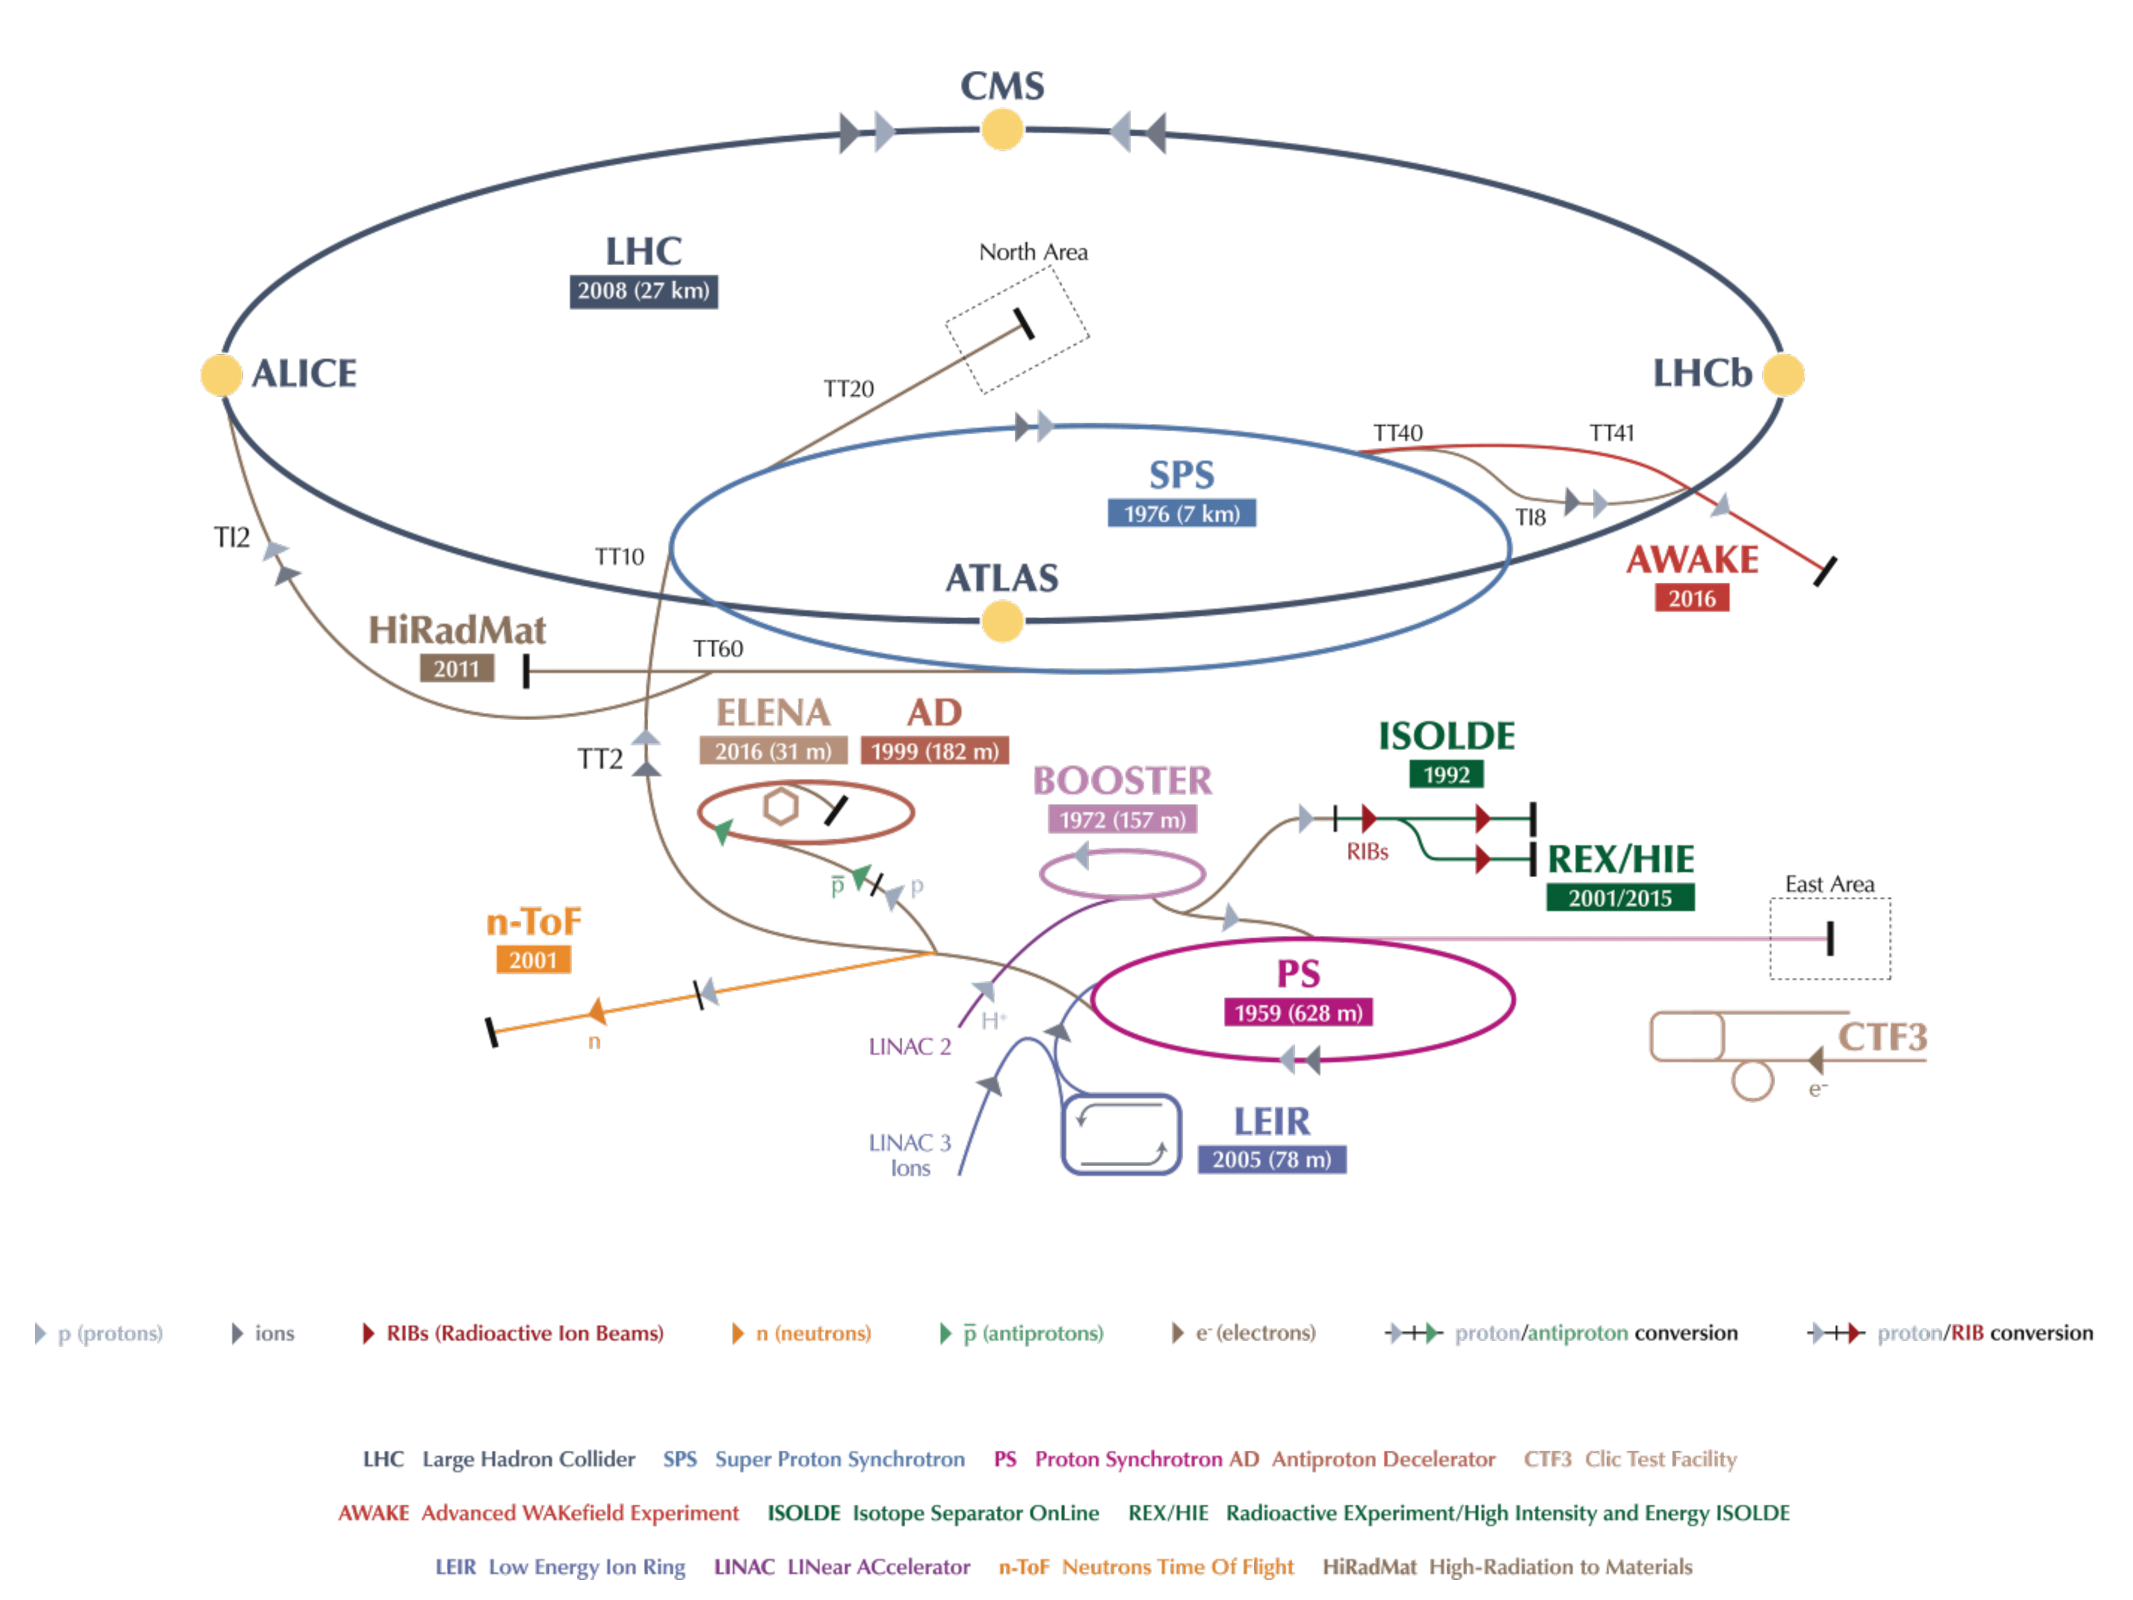
\includegraphics[width=0.72\linewidth]{figures/lhc_lhc.pdf}
\caption{CERN accelerator complex including the four main experiments and the injection chain}
\label{fig:lhc_lhc}
\end{center}
\end{figure}

\vspace{0.3cm}
The beams are injected into the LHC rings for the final acceleration before collisions. There the protons reach the energy of 6.5 TeV after about 20 minutes of acceleration. Nearly 10,000 magnets are used on the LHC. Among them over 1000 superconducting dipole magnets are used to produce a magnetic field of 8.3T and bend the proton beams onto the circular trajectory. Additional, superconducting quadrupole magnets are used to focus the beam, and sextupoles and higher order magnets are used to correct the beam chromaticity.

\vspace{0.3cm}
Inside the LHC particle collisions can happen at 4 interaction points of the tunnel, which correspond to the locations of 4 experiments: CMS, ALICE, ATLAS and LHCb. The ALICE experiment is designed to study quark-gluon plasma using data collected during heavy ion operations of the LHC. These measurements are designed to draw conclusions about the initial state of the universe. LHCb focuses on precisely measuring B-meson decays and CP-violating processes. CMS and ATLAS are the two general purpose experiments at the LHC built for studying a broad range of physics processes. These studies include precision measurements of Standard Model processes and parameters, thereby deepening our knowledge and understanding of the Standard Model. Study of the production and properties of the Higgs boson and searches for physics beyond the Standard Model are major fields of study.

\vspace{0.3cm}
The number of collisions generated at the LHC is proportional to the cross section for proton-proton interactions and the integrated luminosity, and can be written as $N=\sigma \times L$. Here $L$ is the integrated luminosity and is defined as the integral of instantaneous luminosity (denoted by $\mathcal{L}$) over time, as shown in Equation~\ref{eqn:lhc_intelumi}.
\begin{equation}
L=\int \mathcal{L}dt
\label{eqn:lhc_intelumi}
\end{equation}
The maximal instantaneous luminosity of LHC in 2016 reached 15.30 Hz/nb, and the total integrated luminosity delivered by LHC in 2016 was 40.82 fb$^{-1}$. A total of 37.76 fb$^{-1}$ was recorded by CMS and 35.9 fb$^{-1}$ satisfied the data quality requirements used in this analysis. Figure~\ref{fig:lhc_lumi2016} shows the development of instantaneous and integrated luminosity during year of 2016.

\begin{figure}[htbp]
\begin{center}
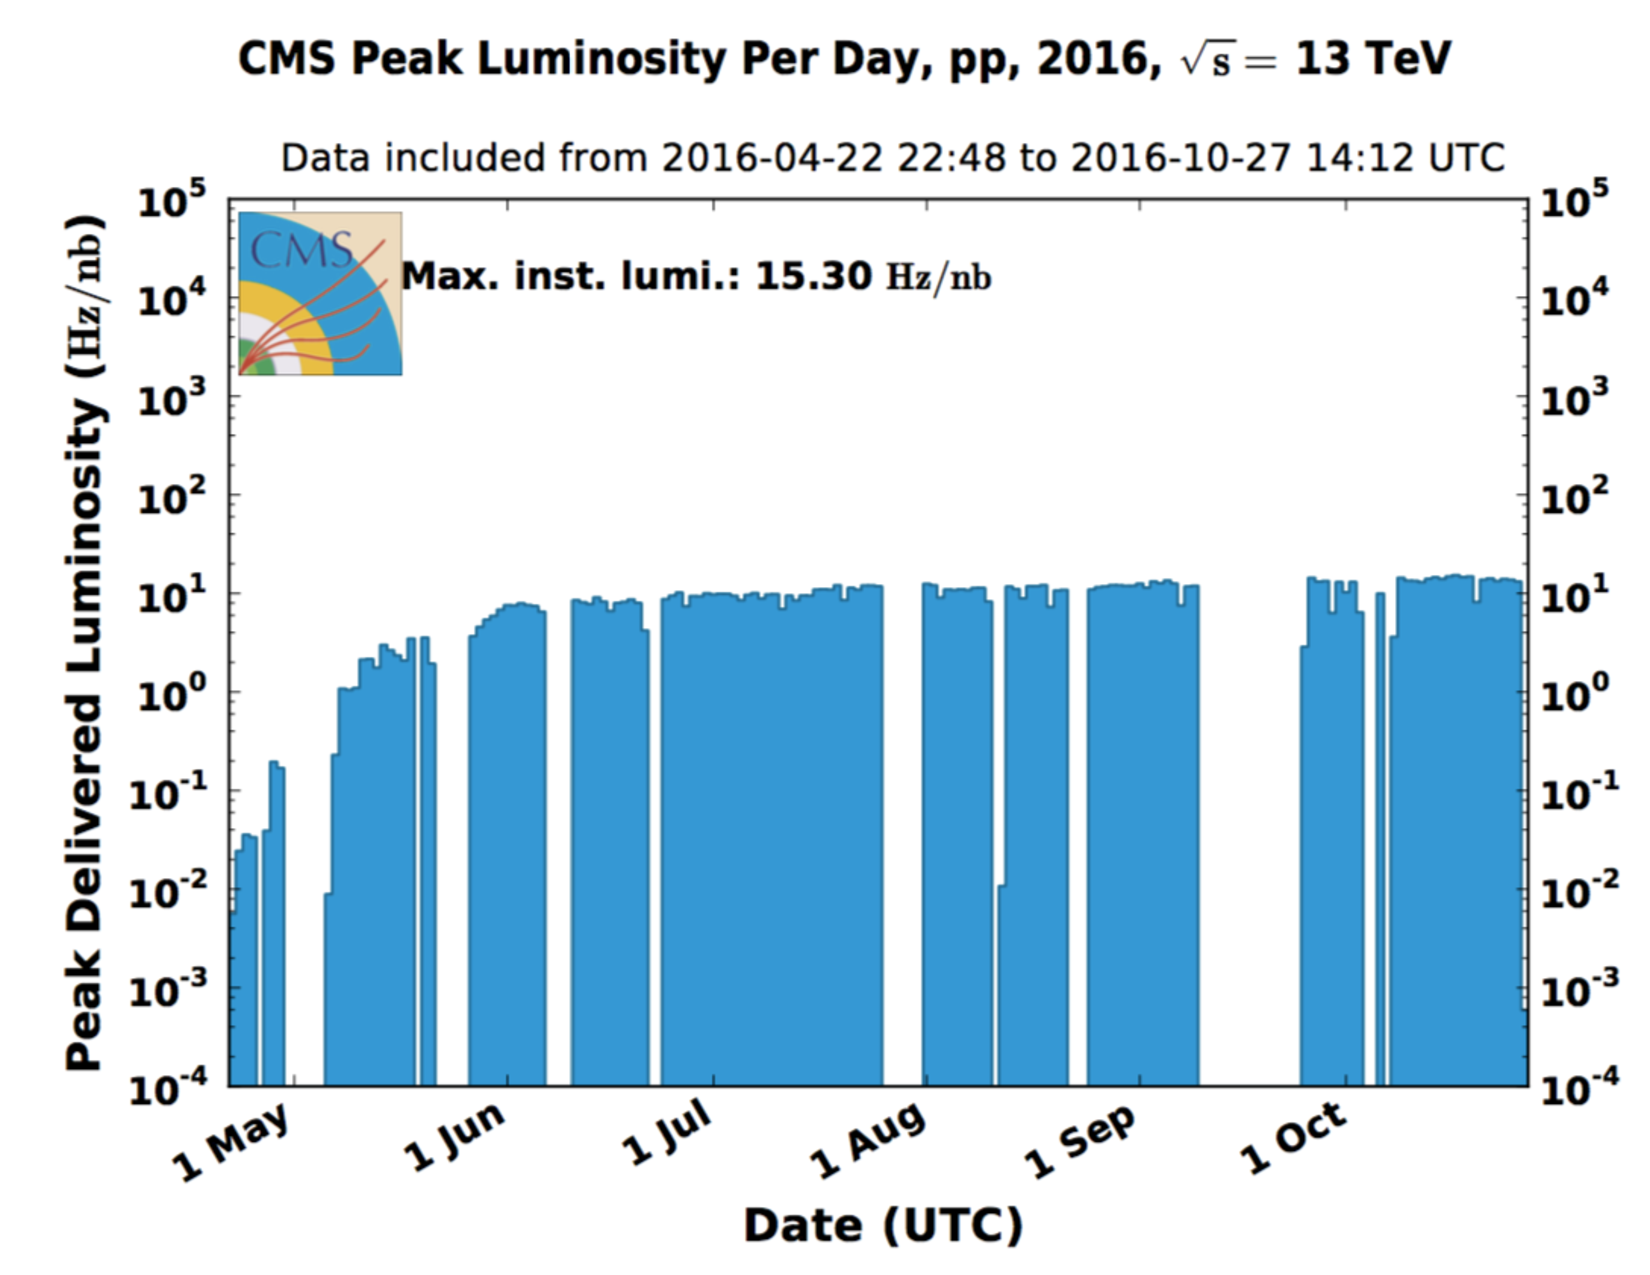
\includegraphics[width=0.49\linewidth, page=1]{figures/lhc_lumi2016.pdf}
\includegraphics[width=0.49\linewidth, page=2]{figures/lhc_lumi2016.pdf}
\caption{Daily peak instantaneous luminosity (left) and integrated luminosity (right) of 2016 LHC proton-proton collisions.}
\label{fig:lhc_lumi2016}
\end{center}
\end{figure}

\section{The Compact Muon Solenoid (CMS) Experiment}
The Compact Muon Solenoid (CMS) detector~\cite{lhc_cmsatcern} is one of the two general purpose detectors at the LHC. It sits 100 meters underground at the LHC interaction point opposite the CERN site, in the French village of Cessy, and measures 15 meters in height, 22 meters in length. And the weight of 14,000 tons makes the CMS detector the heaviest particle physics detector in the world. The CMS detector is designed as a barrel-like detector around the interaction point of the proton beams delivered by the LHC, consisting of multiple layers of subdetectors. The detector can be separated into parts: the central part, ofter referred to as "barrel", and the two sections closing out the barrel on the ends of the detector called "endcaps". 

Figure~\ref{fig:lhc_cmsstructure} shows the structure and components of the CMS detector.
\begin{figure}[htbp]
\begin{center}
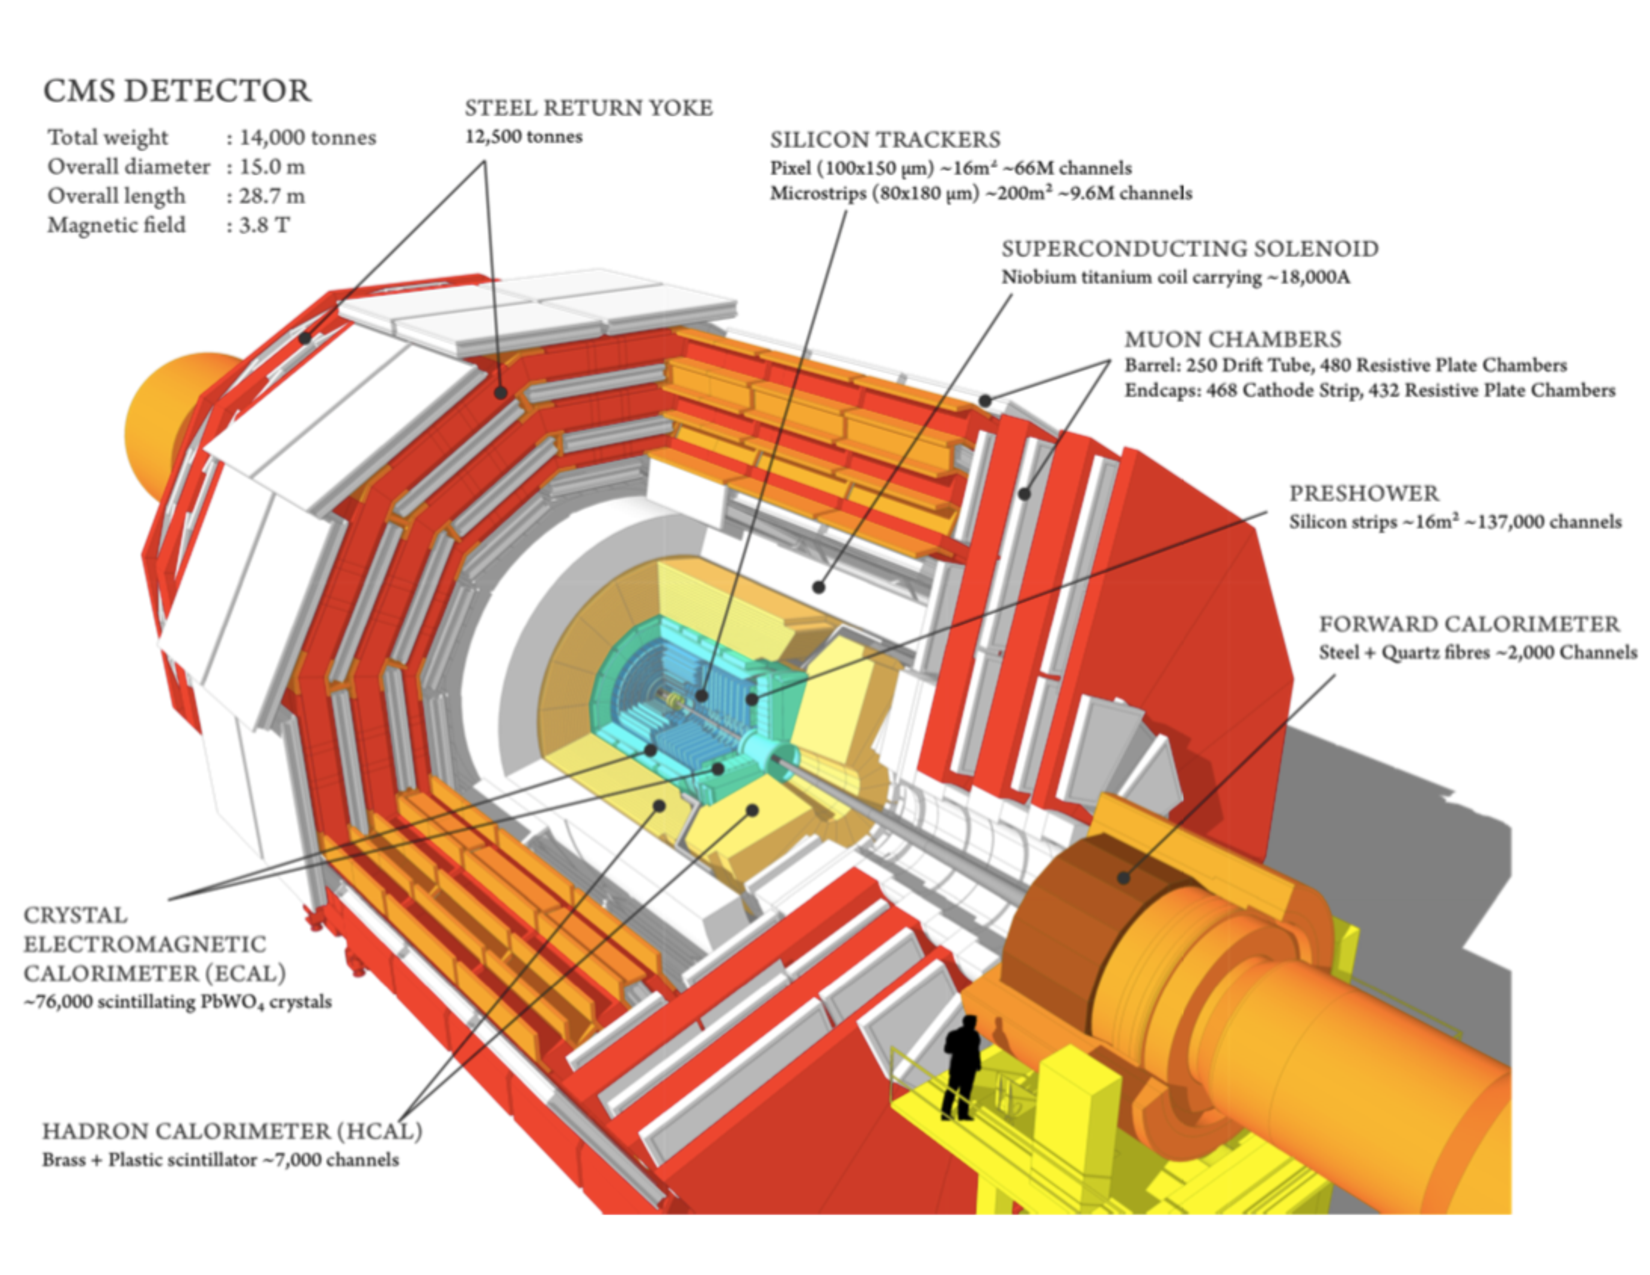
\includegraphics[width=0.7\linewidth, page=1]{figures/lhc_cmsstructure.pdf}
\includegraphics[width=0.7\linewidth, page=2]{figures/lhc_cmsstructure.pdf}
\caption{Illustration of CMS detector structure and subdetectors as components in a cut-out quadrant view (upper), and a cross sectional slice view as well as the trajectories of various particles from p-p collisions in the detector (lower).}
\label{fig:lhc_cmsstructure}
\end{center}
\end{figure}

\vspace{0.3cm}
One characteristic of the CMS detector is its strong axial magnetic field at a uniform strength of 3.8 T, generated by a superconducting solenoid magnet surrounding the inner detector subsystems. Figure~\ref{fig:lhc_magnetdistr} shows the magnetic field distribution measured using cosmic ray tracks~\cite{lhc_magnetmap}. The magnetic field is mostly confined within the steel yoke around the solenoid. Most particles from the collisions except muons would either deposit all their energy in the subdetectors before the yoke or be stopped by the yoke.
\begin{figure}[htbp]
\begin{center}
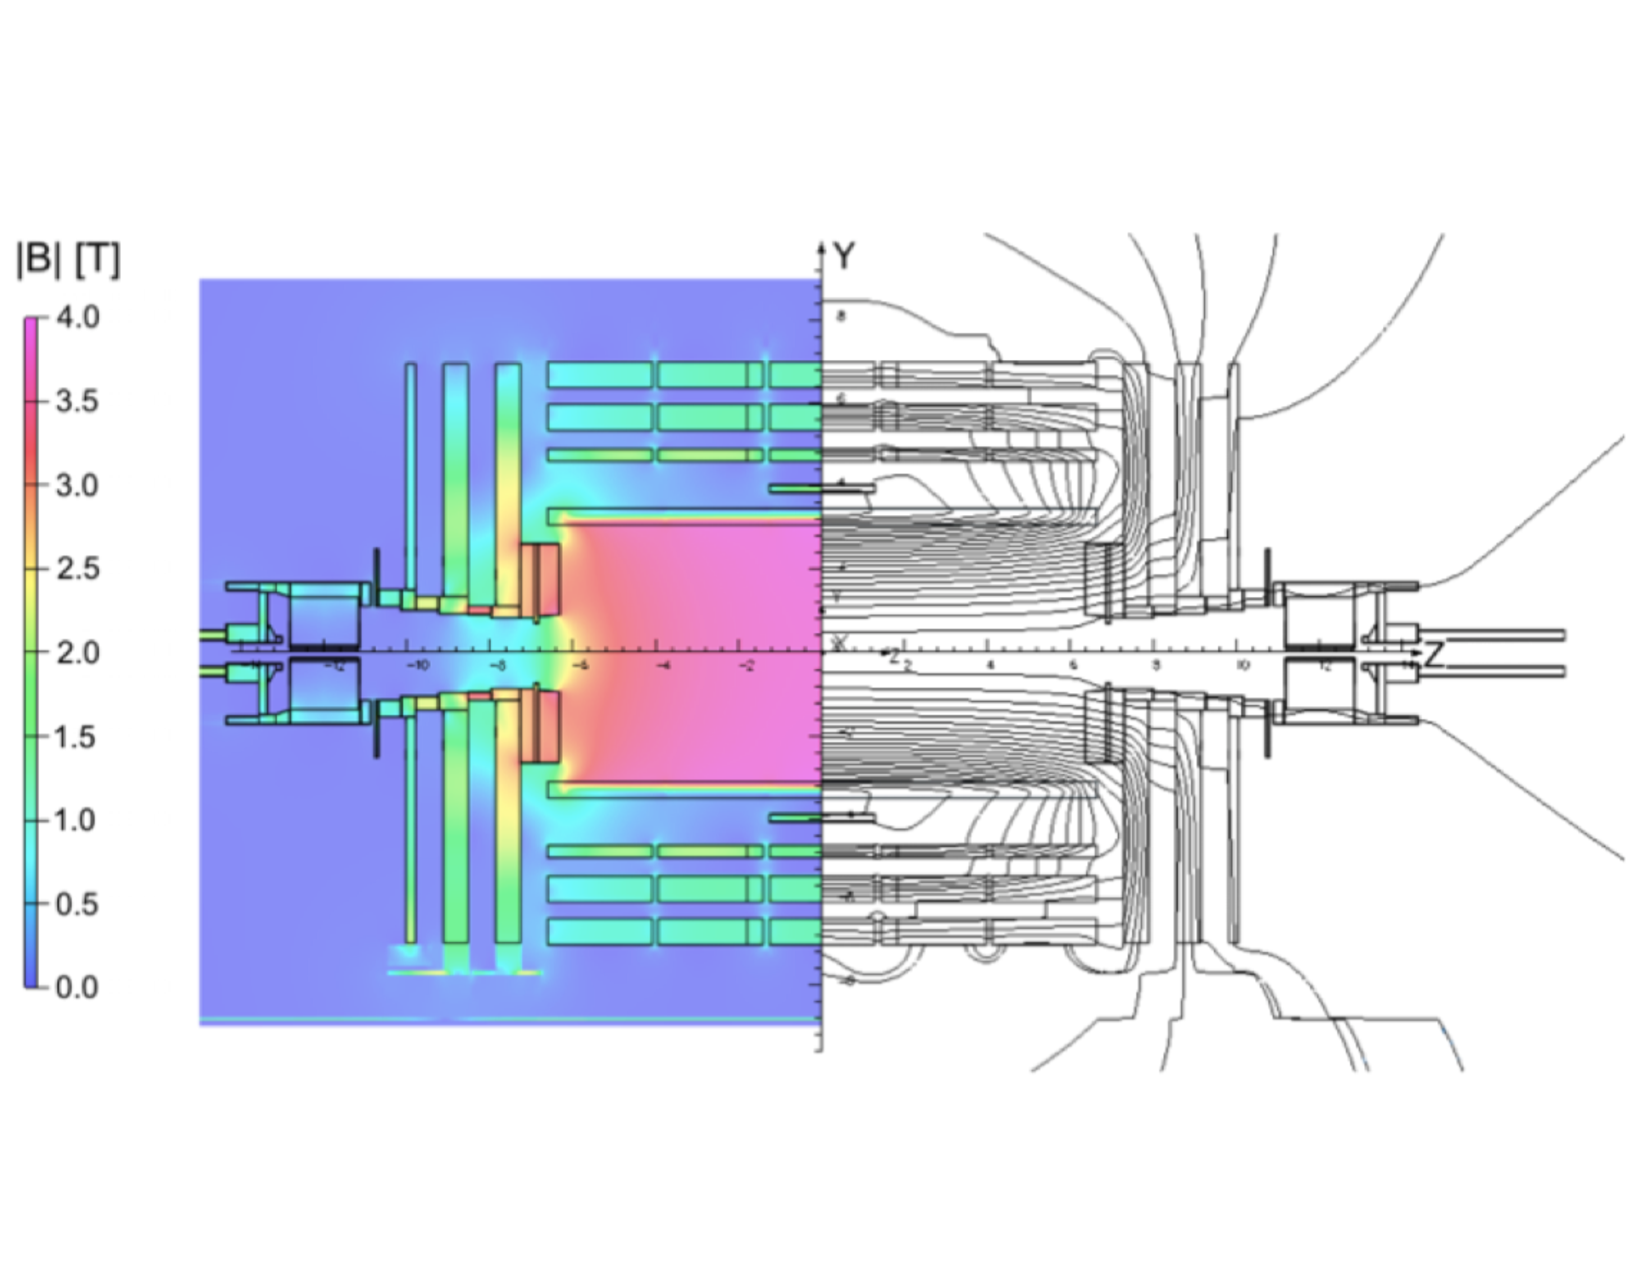
\includegraphics[width=0.7\linewidth, page=1]{figures/lhc_magnetdistr.pdf}
\caption{CMS magnetic field strength (left) and field lines (right)}
\label{fig:lhc_magnetdistr}
\end{center}
\end{figure}

\vspace{0.3cm}
Two sets of coordinate systems are widely used in CMS. One is an orthogonal right handed coordinate system, with the origin sitting at the nominal collision point inside the experiment. The $x$-axis points radially toward the center of the LHC ring, the $y$-axis points upward perpendicular to the LHC ring plane, and the $z$-axis correspondingly points counterclockwise along the beam pipe. Apart from the orthogonal coordinate system, a spherical coordinate system is used due to the cylindrically symmetric design of the detector. Differing from the regular spherical coordinate with parameter $\phi$ denoting the azimuthal angle to the $x$ axis in the $x-y$ plane and parameter $\theta$ denoting the polar angle measured from the $z$ axis, this coordinate in CMS keeps the $\phi$ parameter but uses the pseudorapidity $\eta$ defined in Equation~\ref{eqn:lhc_eta} in the place of $\theta$.
\begin{equation}
\eta = -ln[tan(\frac{\theta}{2})]
\label{eqn:lhc_eta}
\end{equation}

\vspace{0.3cm}
Based on this spherical coordinate, parameter $\Delta R$ is introduced as a measurement of the distance between two particles, and defined as $\Delta R=\sqrt{\Delta\eta^2 + \Delta\phi^2}$
.
\subsection{Inner Tracking System} 
The inner tracking system~\cite{lhc_trackerdesign} is the innermost component of the CMS detector. The main functionality of the inner tracking system is to precisely measure the trajectory of charged particles such as charged leptons and hadrons. It consists of an inner pixel detector and a strip tracker. Figure~\ref{fig:lhc_trackerbarrel} shows the structure of the tracking system
\begin{figure}[htbp]
\begin{center}
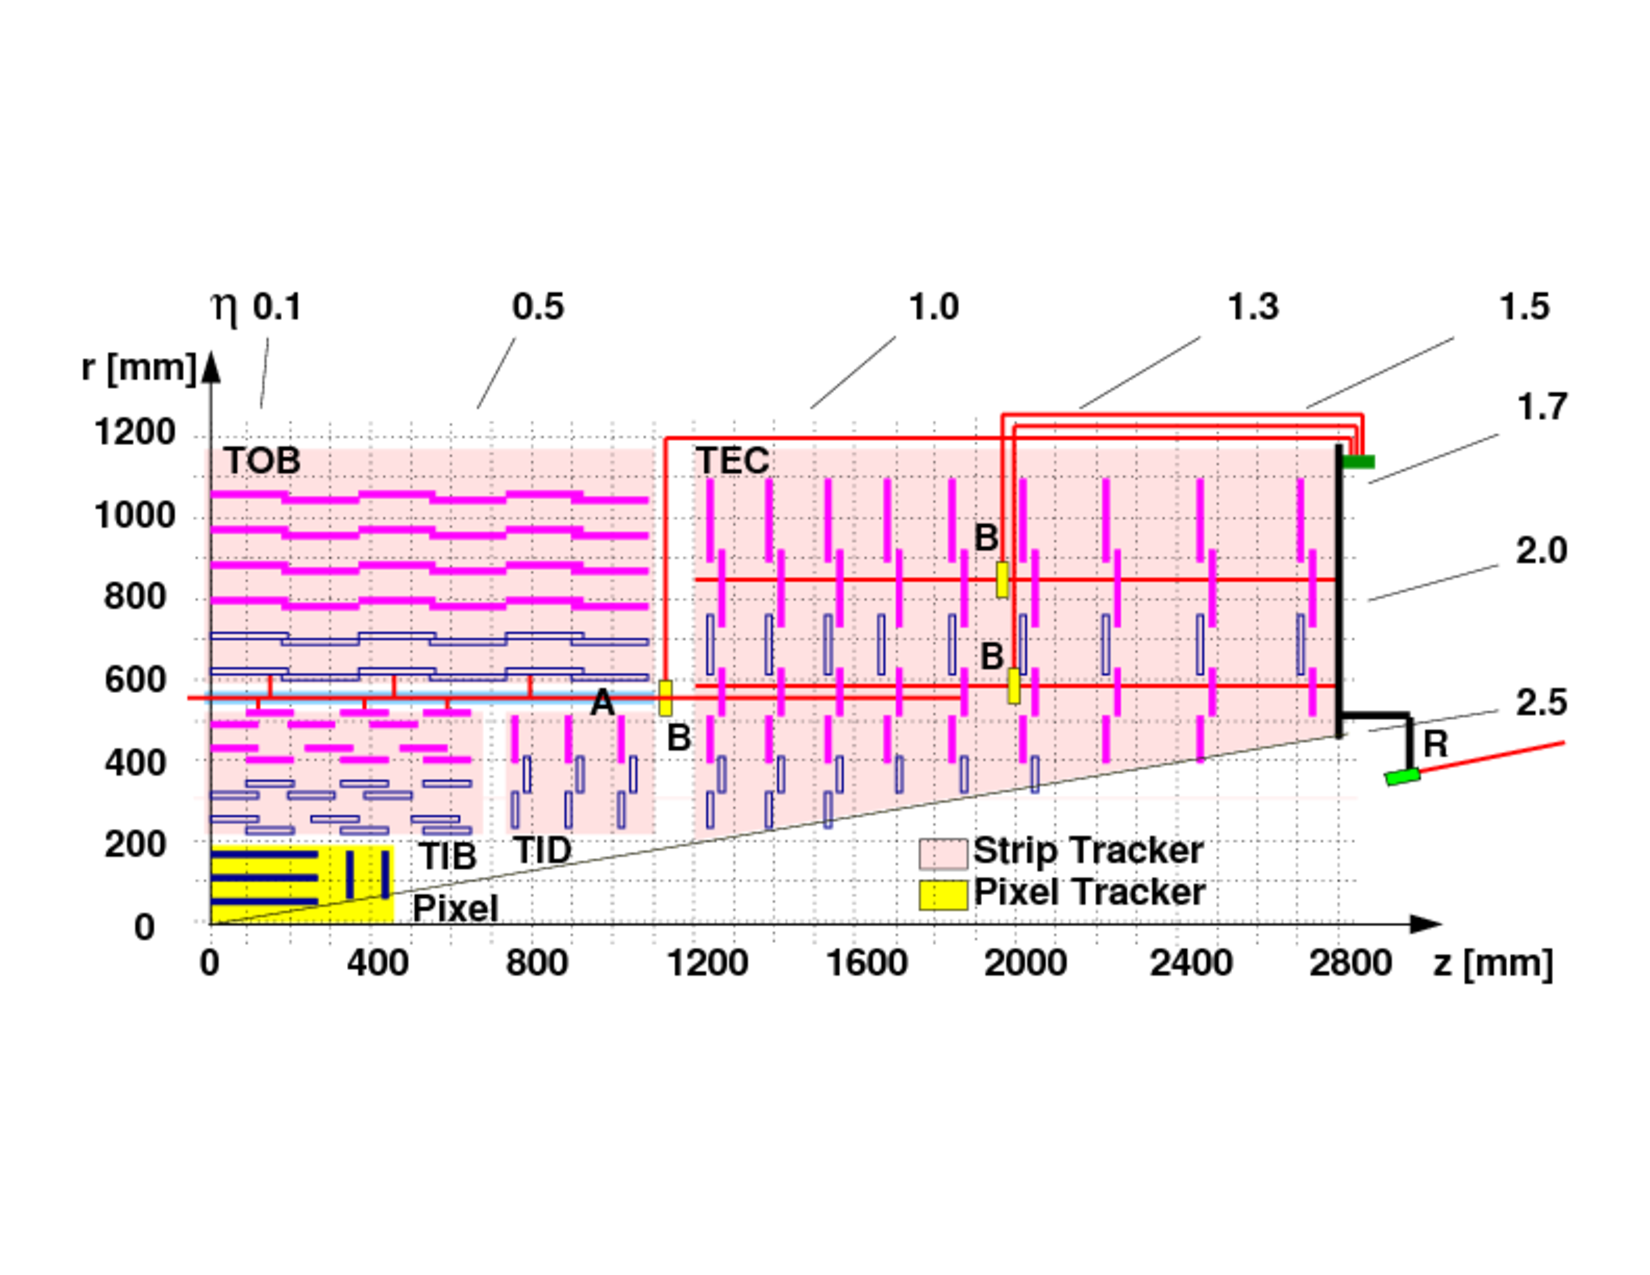
\includegraphics[width=0.7\linewidth, page=1]{figures/lhc_trackerbarrel.pdf}
\includegraphics[width=0.7\linewidth, page=2]{figures/lhc_trackerbarrel.pdf}
\caption{Structure of CMS tracking system in the plane parallel (upper) and perpendicular (lower) to the $z$ axis.}
\label{fig:lhc_trackerbarrel}
\end{center}
\end{figure}

\subsubsection{Inner pixel detector}
The inner pixel detector, consisting of 3 cylindrical layers with minimal radius of 4 cm and disks on each end as endcaps, is the closest detector to the interaction point of the experiment, which makes it vital in reconstructing the tracks of very short-lived particles. But being close to the interactions also means an enormous particle flux. Therefore the pixel detector's design was driven by the goal of getting the best track position resolution possible while also being very radiation tolerant. The inner pixel detector contains 65 million silicon pixel sensors each with a dimension of $100\mu m \times 150\mu m$. These pixel sensors were built using high dose n-implants on a high resistance n-substrate, which ensures high signal collection efficiency with only moderate bias voltages even after high doses of radiation.
\subsubsection{Strip tracker}
After passing through the pixel detector, particles reach the outer silicon strip tracker at radius of 130 cm. The strip detector consists of the Tracker Inner Barrel (TIB), Tracker Inner Disks (TID), Tracker Outer Barrel (TOB), and the Tracker End Caps (TEC). The TIB contains 4 layers of silicon sensors, among which the inner 2 layers are built with double sided sensors while the other 2 layers are single sided. The TID, placed on each end of TIB as the endcaps, is composed of 2 sets of disks of sensors, with 3 disks in each set. Surrounding the inner tracker is the TOB, consisting of 6 layers. The inner 2 layers carry double sided sensors. Finally the endcaps (TEC) close off the tracking system, with 9 disks of sensors on each side. 

\vspace{0.3cm}
The CMS tracking system covers the detector region up to $|\eta| = 2.5$ and has a resolution of up to 10 $\mu m$ in the $x-y$ direction and 20 $\mu m$ in the $z$ direction. 

\subsection{Electromagnetic Calorimeter} 
The Electromagnetic Calorimeter (ECAL)~\cite{lhc_ecaldesign} is designed mainly for the measurement of the energy of photons and electrons. It sits between the tracker and the Hadron Calorimeter, covering the $\eta$ range from -3.0 to 3.0. The ECAL is composed of the ECAL Barrel (EB), ECAL Endcaps (EE) and ECAL Preshower (ES). Figure~\ref{fig:lhc_ecal} shows the structure of ECAL.
\begin{figure}[htbp]
\begin{center}
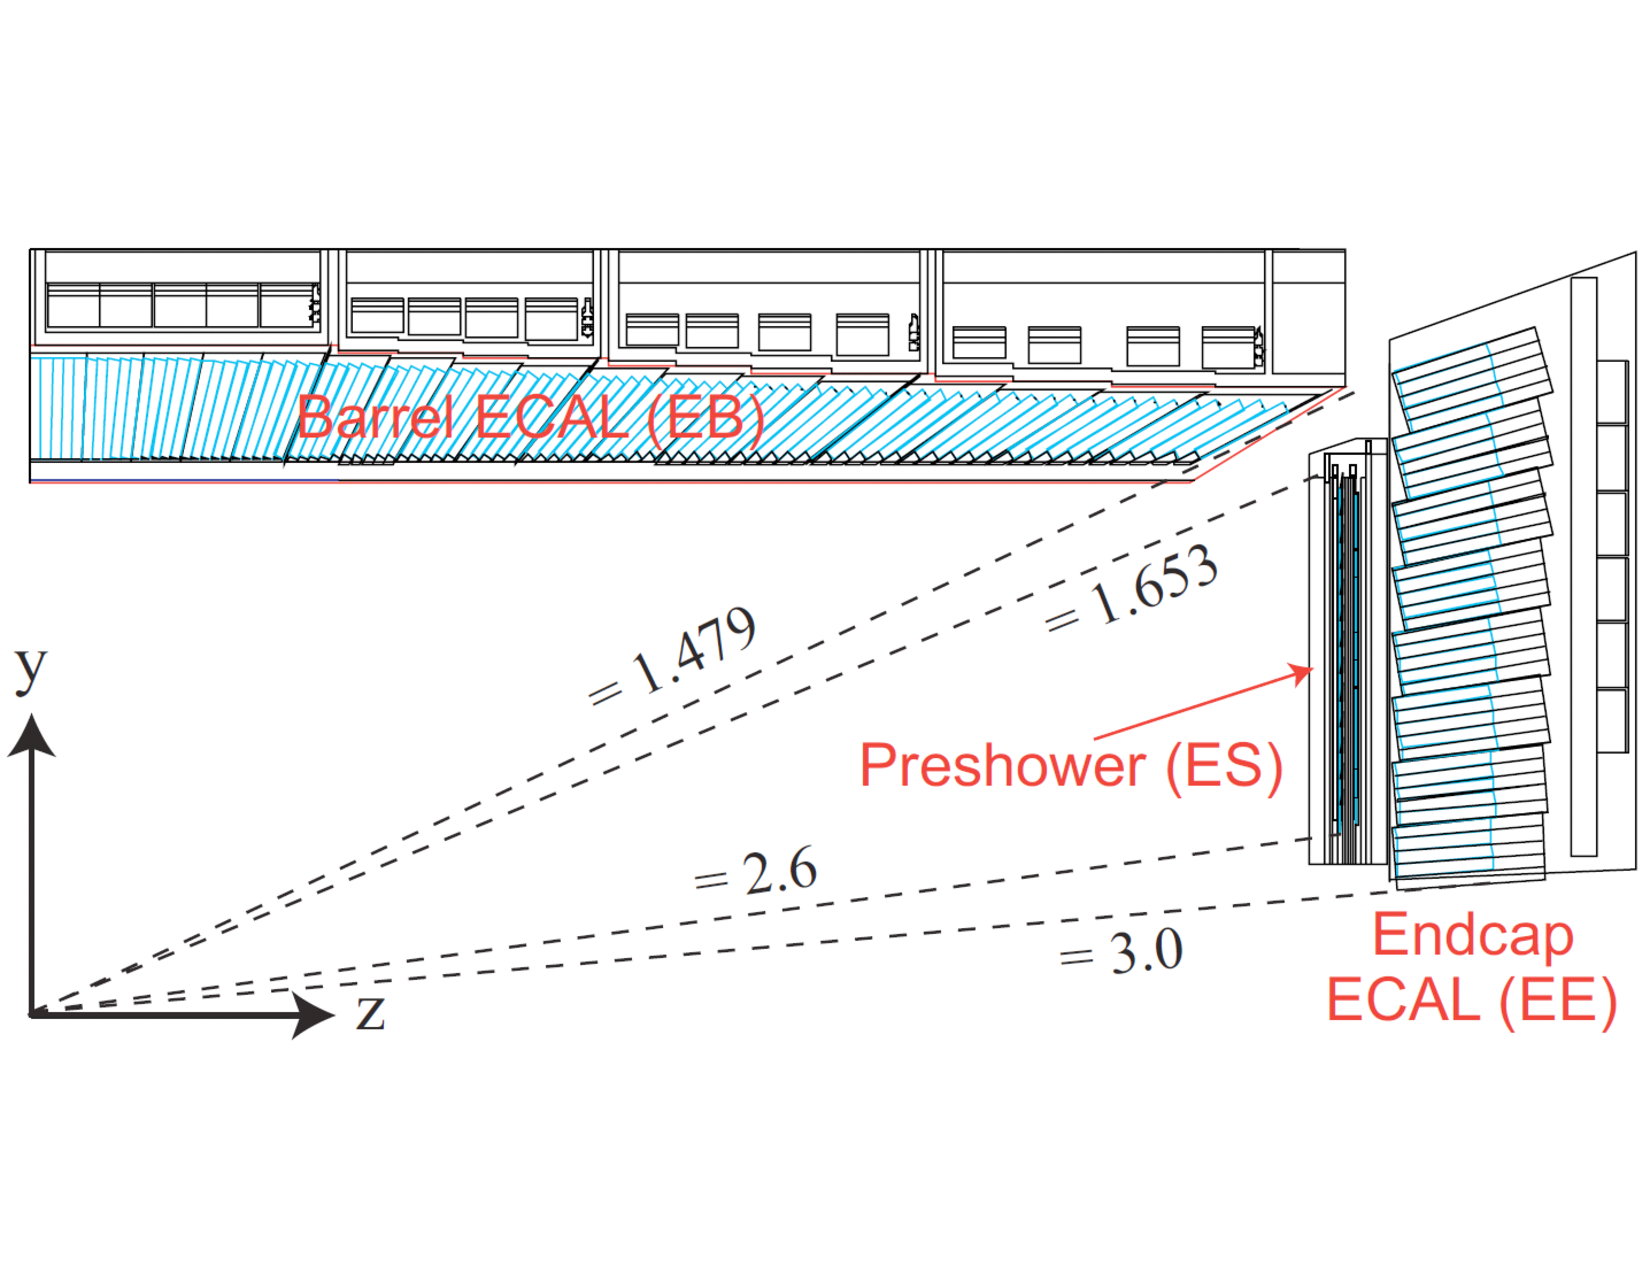
\includegraphics[width=0.7\linewidth]{figures/lhc_ecal.pdf}
\caption{Structure of the Electromagnetic Calorimeter (ECAL) in the $y-z$ plane.}
\label{fig:lhc_ecal}
\end{center}
\end{figure}

\subsubsection{ECAL Barrel and Endcap}
ECAL Barrel and Endcap contains near 80,000 lead tungstate (PbWO4) crystals each with face dimension of approximately $3cm\times 3cm$. These crystals are primarily composed of metal with high density, and have good radiation tolerance and short radiation length. This material produces scintillation light with fast photon showers. The lead tungstate crystals provide precise energy resolution and allow the calorimeter to be compact enough for the CMS design. However, a drawback of the crystal is that its light yield strongly depends on temperature. The nominal operating temperature of the ECAL is maintained at $18^{\circ}C$, with variation within $0.1^{\circ}C$, for the desired energy measurement resolution. 

\vspace{0.3cm}
The EB consists of over 60,000 crystals and covers $|\eta|$ up to 1.479. Avalanche photodiodes (APD) are mounted on the rear face of these crystals to collect the scintillation light and amplify the signal. Each of the two endcaps contains over 7,000 crystals. The crystals are grouped in $5\times 5$ arrays referred to as "super crystals". Vacuum phototriodes (VPT) are glued to these crystals for signal collection and amplification, similar to the APDs in the EB. The EE covers the $|\eta|$ range between 1.479 and 3.0. 

\subsubsection{ECAL Preshower}
The ECAL Preshower (ES) detectors sit in front of the EEs. They are composed of two planes of lead followed by silicon sensor strips. When photons pass through, electromagnetic showers are produced in the lead layer, and then detected by the silicon sensors. The silicon sensor strips on the ES with width of 2mm give much better position resolution, compared to the $3cm\times 3cm$ ECAL crystals, and can distinguish individual photons in the adjacent photon pairs from $\pi^{0}$ decays.

\subsection{Hadronic Calorimeter} 
The Hadron Calorimeter (HCAL)~\cite{lhc_hcaldesign} is designed for the measurement of energy of the hadrons produced from the p-p collisions, and plays a crucial role in the indirect measurement of particles having no interaction with the detector, such as neutrinos. The HCAL can be divided into 4 components, which are the HCAL Barrel (HB), HCAL Endcaps (HE), HCAL Forward calorimeter (HF) and HCAL Outer calorimeter (HO). Figure~\ref{fig:lhc_hcaldesign} shows the structure of the HCAL detector.
\begin{figure}[htbp]
\begin{center}
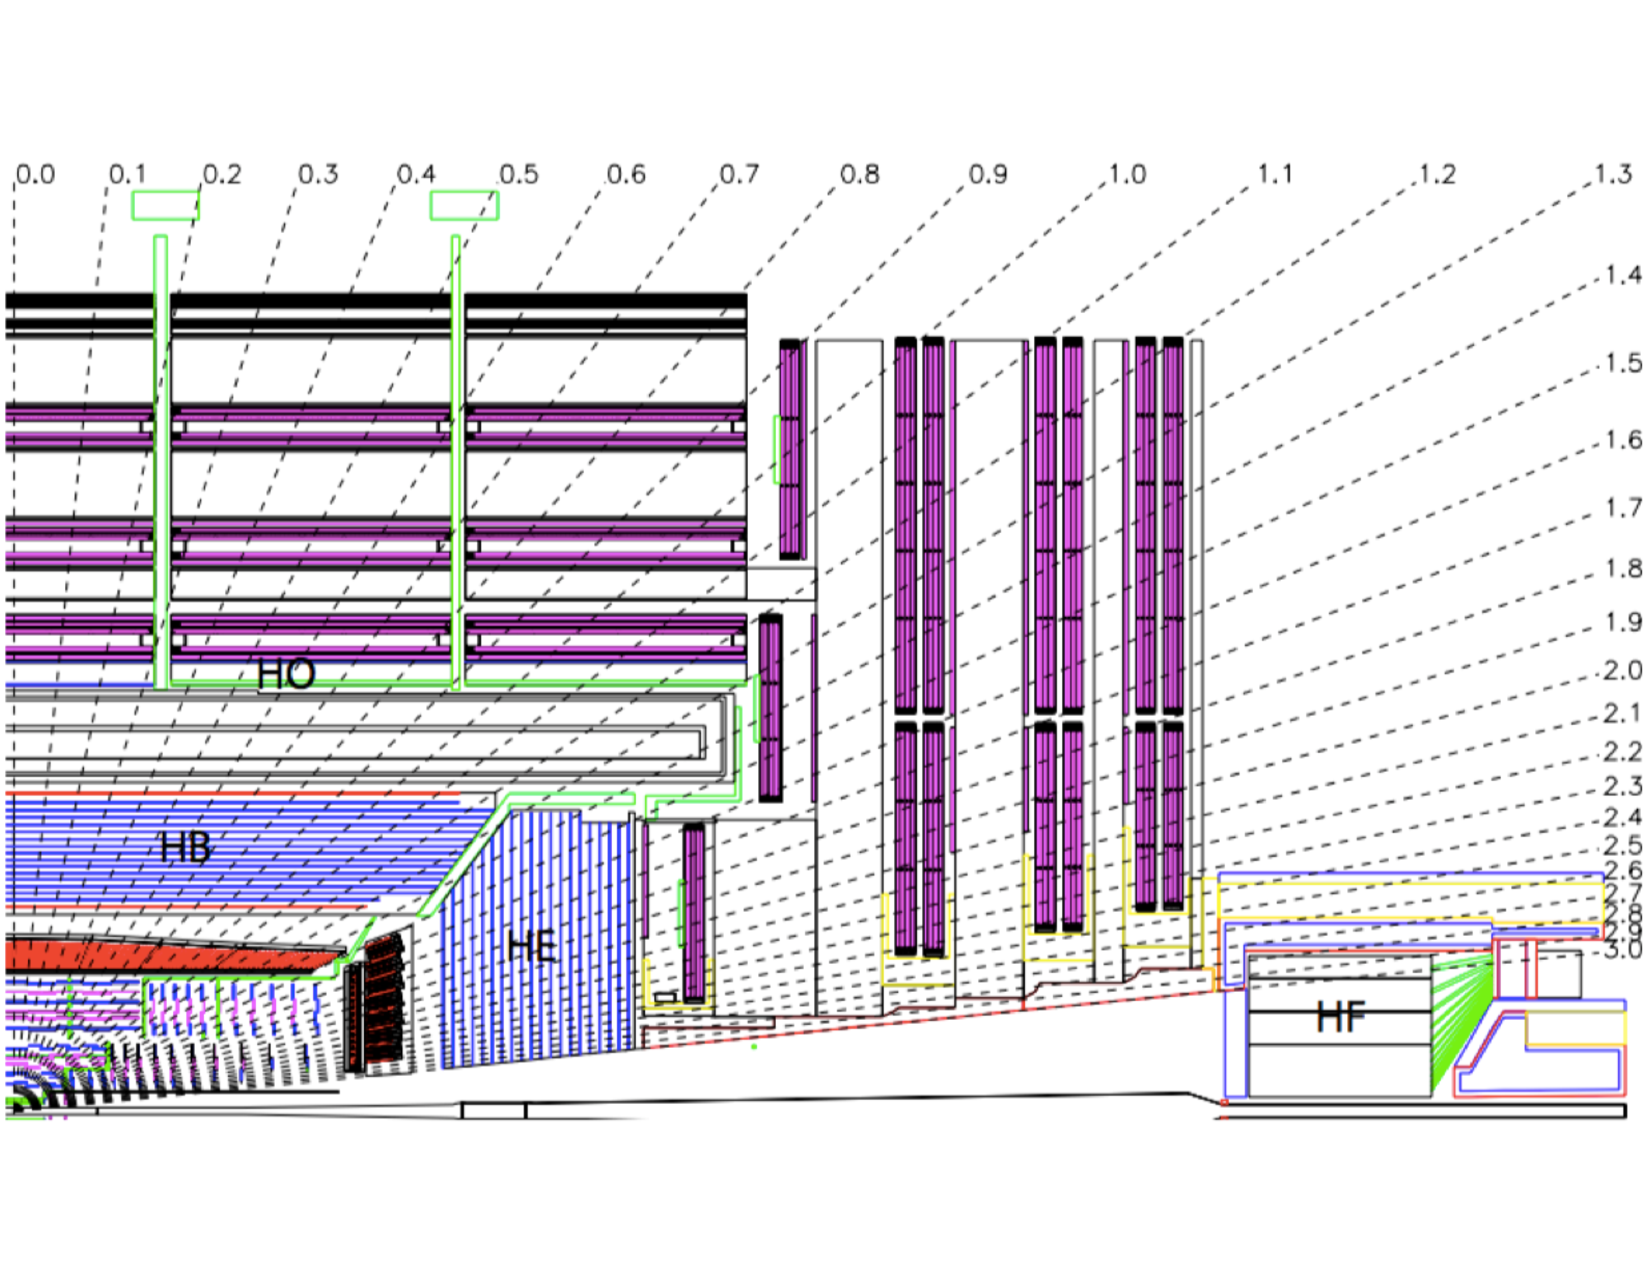
\includegraphics[width=0.7\linewidth]{figures/lhc_hcaldesign.pdf}
\caption{Structure of the Hadron Calorimeter (HCAL) in the $y-z$ plane. Muon Chambers are also shown to illustrate the position of HF.}
\label{fig:lhc_hcaldesign}
\end{center}
\end{figure}

\subsubsection{HCAL Barrel and Endcap}
The HB and HE are located inside the solenoid magnet, surrounding the ECAL. Unlike ECAL which is built completely by crystals, HB and HE are sampling calorimeters made of alternating layers of metal as absorbers and tiles of Kuraray SCSN81 plastic scintillator. When a particle passes through the absorbers, numerous secondary particles are produced. The particle shower produced in the absorbers causes the scintillator layers to emit violet light. This violet light is then shifted into green light in wavelength-shifting fibers and carried to the readout boxes by clear fibers, where the light is converted into fast electronic signals by Hybrid Photodiodes (HPDs) photosensors.

\vspace{0.3cm}
The absorber material for HB is steel for the innermost and outermost layers and brass for the layers in between. The HB consists of 2 halves, referred to as HB Plus (HBP) and HB Minus (HBM). They each contains 18 $\phi$ sections called wedges. Each wedge weighs 26 tonnes and is further subdivided in 4 $\phi$ sectors and 16 $\eta$ sectors. The HB covers the $|\eta|$ up to 1.3.

\vspace{0.3cm}
Like the HB, the endcaps are made of alternating brass layers and Kuraray SCSN81 plastic scintillator layers. Each HE is divided into 36 $\phi$ sectors and 13 $\eta$ towers. The HE covers $|\eta|$ between 1.3 and 3.0.

\subsubsection{HCAL Outer Calorimeter}
The HO sits outside the magnet coil and covers the region of $|\eta|<1.3$. It consists of a single 10 mm Bicron BC408 scintillator layer at a radial distance of 4.07 m. Like the HB and HE, the scintillation light is collected by wavelength-shifting fibers and sent to HPDs by clear fibers. The HO expands the radial sampling depth of the HCAL system and ensures no energy leakage undetected by HB.

\subsubsection{HCAL Forward Calorimeter}
The HFs are placed outside the muon system, 11.2m away from the interaction point of the experiment along the $z$-axis on each side. The HF receives a great amount of radiation from the collision due to its position and thus has to be more resistant to radiation than the rest of HCAL components. Each HF is made of steel, shaped as a cylinder. The steel in this case works as absorbers while radiation-hard quartz fibers are placed along grooves inside, 5.0 mm apart, and working as Cherenkov radiators. The cylinder has height of 165 cm, outer radius of 130.0 cm, and inner radius of 12.5 cm for the beams to pass through. The HF extends the $|\eta|$ coverage of HCAL to 5.0.

\subsection{Muon System} 
Unlike other particles, muons can penetrate the calorimeters and yoke without being stopped. The CMS muon system aims at the identification and measurement of muons~\cite{lhc_muondesign}. The muon system is the outermost layer of the CMS detector system, and is the largest subdetector in CMS. It includes 1400 muon chambers, which can be categorized into 3 groups: Drift Tubes (DT), Cathode Strip Chambers (CSC) and Resistive Plate Chambers (RPC). The muon system covers the region $|\eta|<2.4$. Figure~\ref{fig:lhc_muon} shows the structure of the muon system.
\begin{figure}[htbp]
\begin{center}
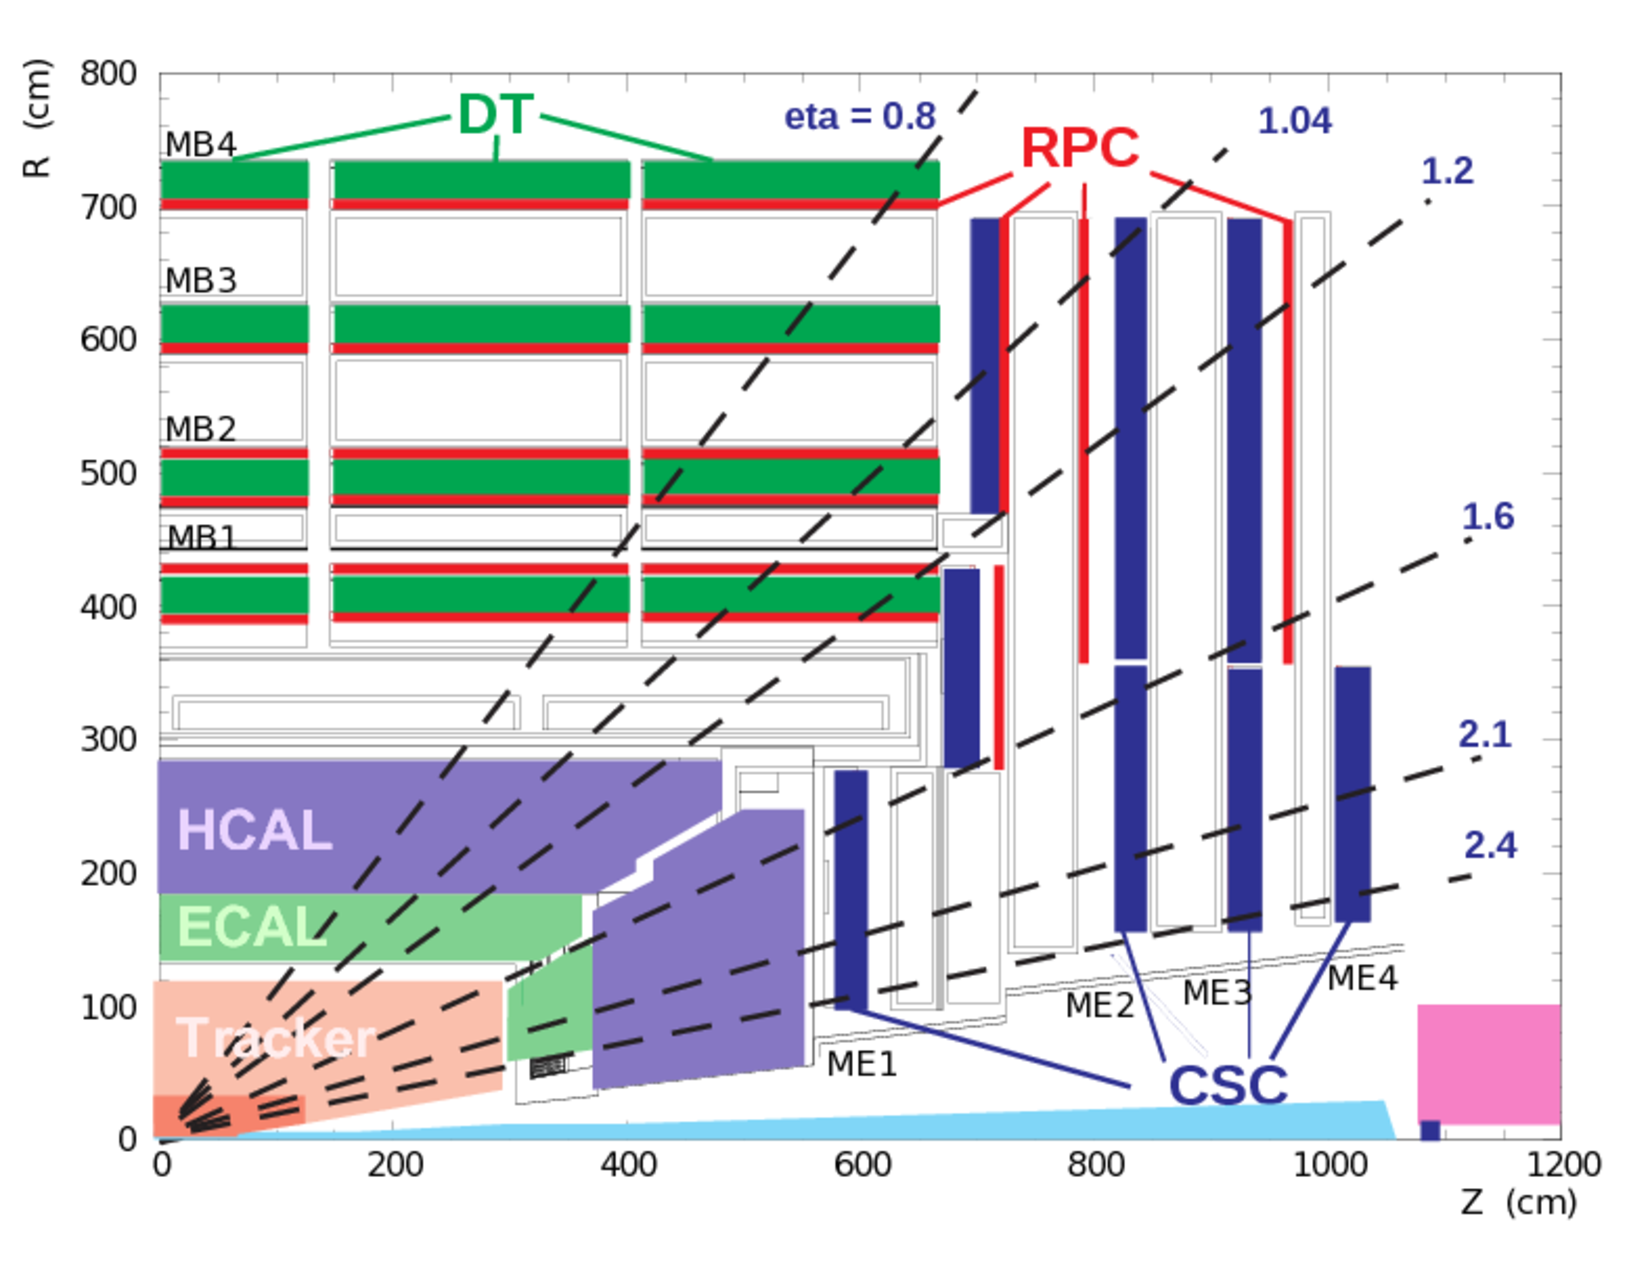
\includegraphics[width=0.7\linewidth]{figures/lhc_muon.pdf}
\caption{Structure of CMS muon system in the $y-z$ plane.}
\label{fig:lhc_muon}
\end{center}
\end{figure}

\subsubsection{Drift Tubes}
The Drift Tubes are used in the barrel of the muon system, and cover the region of $|\eta|<1.2$ with four layers called stations. The inner 3 stations each contain three super layers (SL) with four chambers of DTs filled with a gas mixture of $85\%$ $Ar$ and $15\%$ $CO_{2}$. The outer two SLs provide precise $\phi$ measurements while the middle one measures $\eta$. The outermost station has only two SLs each measuring either $\phi$ or $\eta$.

\subsubsection{Cathode Strip Chambers}
The Cathode Strip Chambers make up the endcap region of the muon system covering $|\eta|$ between $0.9$ and $2.4$. A CSC covers $10-20^{\circ}$ in $\phi$. It consists of 7 cathode strip panels alternating with 6 layers of anode wire planes, filled with a gas mixture of $40\%$ $Ar$, $50\%$ $CO_{2}$ and $10\%$ $CF_{4}$. The cathode strips are arranged in the radial direction to give the measurement of $\phi$, while the anode wires are wound in the $\phi$ direction for radial position measurements.

\subsubsection{Resistive Plate Chambers}
In addition to DTs and CSCs, RPCs are embedded in both the barrel and endcap for $|\eta|$ up to 2.1. Despite of their coarse spatial resolution, RPCs provide very precise timing measurement of muons and are used to supplement the muon triggering system. An RPC is composed of an anode and a cathode as two parallel plates, filled with a gas mixture of $95.2\%$ Freon, $4.5\%$ isobutane, as well as $0.3\%$ hexafluoride and water vapor.

\subsection{Data Acquisition and Trigger System} 
Proton-proton collisions take place every 25 ns with an average of 20 proton-proton interactions per bunch crossing, leading to an input data rate of nearly 1 GHz seen by the CMS detector. However, it is impossible to record and store all the information as the computing system can only handle events up to 400 Hz. Therefore a trigger system is needed for fast processing to select the most interesting events. In CMS a two-stage trigger system is used~\cite{lhc_cmstrigger}: the $Level\; 1\; trigger$ (L1T) and $High\; Level\; trigger$ (HLT).

\subsubsection{Level 1 Trigger}
The $Level\; 1\; trigger$ is the first stage of CMS trigger system. It makes decisions completely based on the coarse information from the calorimeters and muon detectors, allowing for fast response. Local trigger information and decisions are first calculated by each subsystem and then sent to the Global Trigger (GT) where a final decision is made for L1T based on the subsystem information.

\vspace{0.3cm}
The L1T reduces the event rate to 100kHz before sending data on to the $High\; Level\; trigger$.

\subsubsection{High Level Trigger}
The $High\; Level\; trigger$ is entirely software based and relies much more on the reconstruction of physics objects than L1T. This is similar to the offline object reconstructions, but is implemented in a simpler and faster way. This allows the HLT to define events based on physics objects and to select those that are most interesting for data analysis. A dedicated computing farm is used for the HLT processing.

\vspace{0.3cm}
The HLT brings the event rate down to the order of 100 Hz. Events selected by the HLT are kept and sent to the data storage system to await offline processing.

